\subsection{Fase 1: Inicialización de Soluciones} \label{sec:3:inicializacion-soluciones}

La fase de inicialización toma como entrada la planificación inicial, la planificada para el día y que ya no tiene validez debido a la incidencia; junto a los datos relativos a la incidencia que son:

\begin{itemize}
	\item Hora a la que se produce la incidencia.
	\item Tipo de incidencia.
	\item Si la incidencia es por un cambio imprevisto de sectorización, la nueva sectorización.
	\item Si la incidencia es por una baja de un trabajador, hora de la baja y los datos del trabajador y, opcionalmente, hora del alta y datos del trabajador (puede ser el mismo u otro que no forme parte del turno inicial).
\end{itemize}

\begin{figure}[htbp]
	\centering
	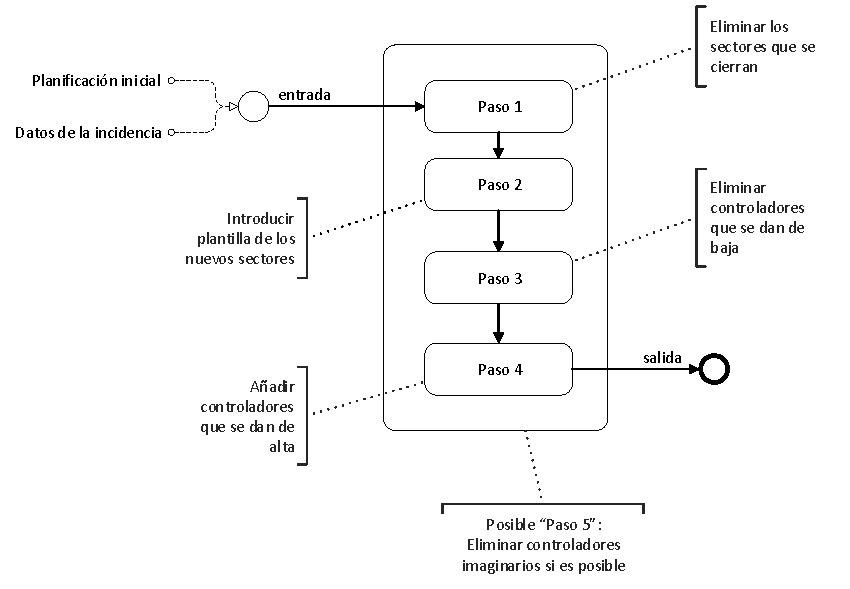
\includegraphics[width=\linewidth]{Esquema-Fase-1-extendido}
	\caption{Diagrama de flujo del funcionamiento de la Fase 1}
	\label{fig:3:esquema-fase-1}
\end{figure}

Con esos datos, la \faseuno{} deberá convertir la planificación inválida en una \textit{solución inicial}, que 
emplearemos como punto de partida para el sistema de búsqueda inteligente que es la \fasedos{}. Para ello distinguimos dos tipos de tareas, las relativas a la incidencia por cambio de sector (pasos 1 y 2) y las relativas a las bajas y altas de los trabajadores (pasos 3 y 4). Los pasos pueden verse esquemáticamente en la \autoref{fig:3:esquema-fase-1}.
Adicionalmente, un quinto paso fue planteado para poder facilitar la tarea de la \fasedos{}, que consistía en reducir el número de controladores añadidos artificialmente en los pasos anteriores moviendo carga de trabajo a otros que la soporten heurísticamente. Finalmente no fue implementada y fue añadida como trabajo futuro.

En la figura \autoref{fig:3:ejemplo-distribucion-inicial} se muestra cómo sería una posible planificación inicial. En este caso ha sido creada en base a \textit{plantillas} o \textit{estadillos}, que es el método empleado habitualmente por el personal para crear la planificación. Consiste en la repetición de un patrón conformado por tres 
controladores para un sector, en el que se suceden trabajo en puesto planificador, trabajo en puesto ejecutivo y descanso con un desfase en incremento para cada controlador, forma que en cada instante de tiempo (imagínese una línea transversal) habrá un controlador en puesto ejecutivo, otro en planificador y otro descansado. \gls{CRIDA} sabe que el uso de estas plantillas si bien no es lo más óptimo es lo más cómodo tanto para la creación manual de la planificación como de cara a no incumplir las restricciones de cada trabajador (ver %TODO: referencias!!).
En las representaciones realizadas, se utilizan identificadores de tres letras en lugar del nombre completo del sector para abreviar y mantener el número de caracteres contante y se han añadido también colores para una mejor visualización.
\textbf{Las letras en mayúscula (AAA-ZZZ) representan un trabajo en puesto de ejecutivo, mientras que las letras minúsculas (aaa-zzz) indican un trabajo en puesto planificador. Los descansos se representan mediante unos (111).}.
Hemos agrupado slots contiguos tanto de trabajo como de descanso idénticos, de manera que visualmente sea más cómodo de entender. Para que las soluciones aquí presentadas tengan validez final, deberíamos añadir indicadores de las horas de los cambios de puesto, sin embargo para este documento esto no es realmente importante por lo que podemos omitirlo.

El tipo de plantilla descrito se le denomina $3\times1$ (3 controladores para 1 sector) pero existen otros tipos como $8\times3$ o $4\times1$, no obstante, la más importante para el sistema es la $3\times1$, que será empleada durante esta Fase.

\subsubsection{Paso 1: Eliminar sectores que se cierran}
El primer paso es el encargado de eliminar los sectores que se cierran. Pongamos por ejemplo que tenemos una 
sectorización 5A que pasa a ser una 6C en un momento dado, tal y como se ilustra en la 
\autoref{fig:3:ejemplo-cambio-sectorizacion}. Como ya hemos dicho previamente, nosotros partimos de una planificación inicial como la representada en la \autoref{fig:3:ejemplo-distribucion-inicial}, que con la nueva sectorización queda totalmente inutilizada, pues podemos ver sectores que ya no se encuentran abiertos a partir del punto de cambio.

\begin{figure}[htbp]
	\centering
	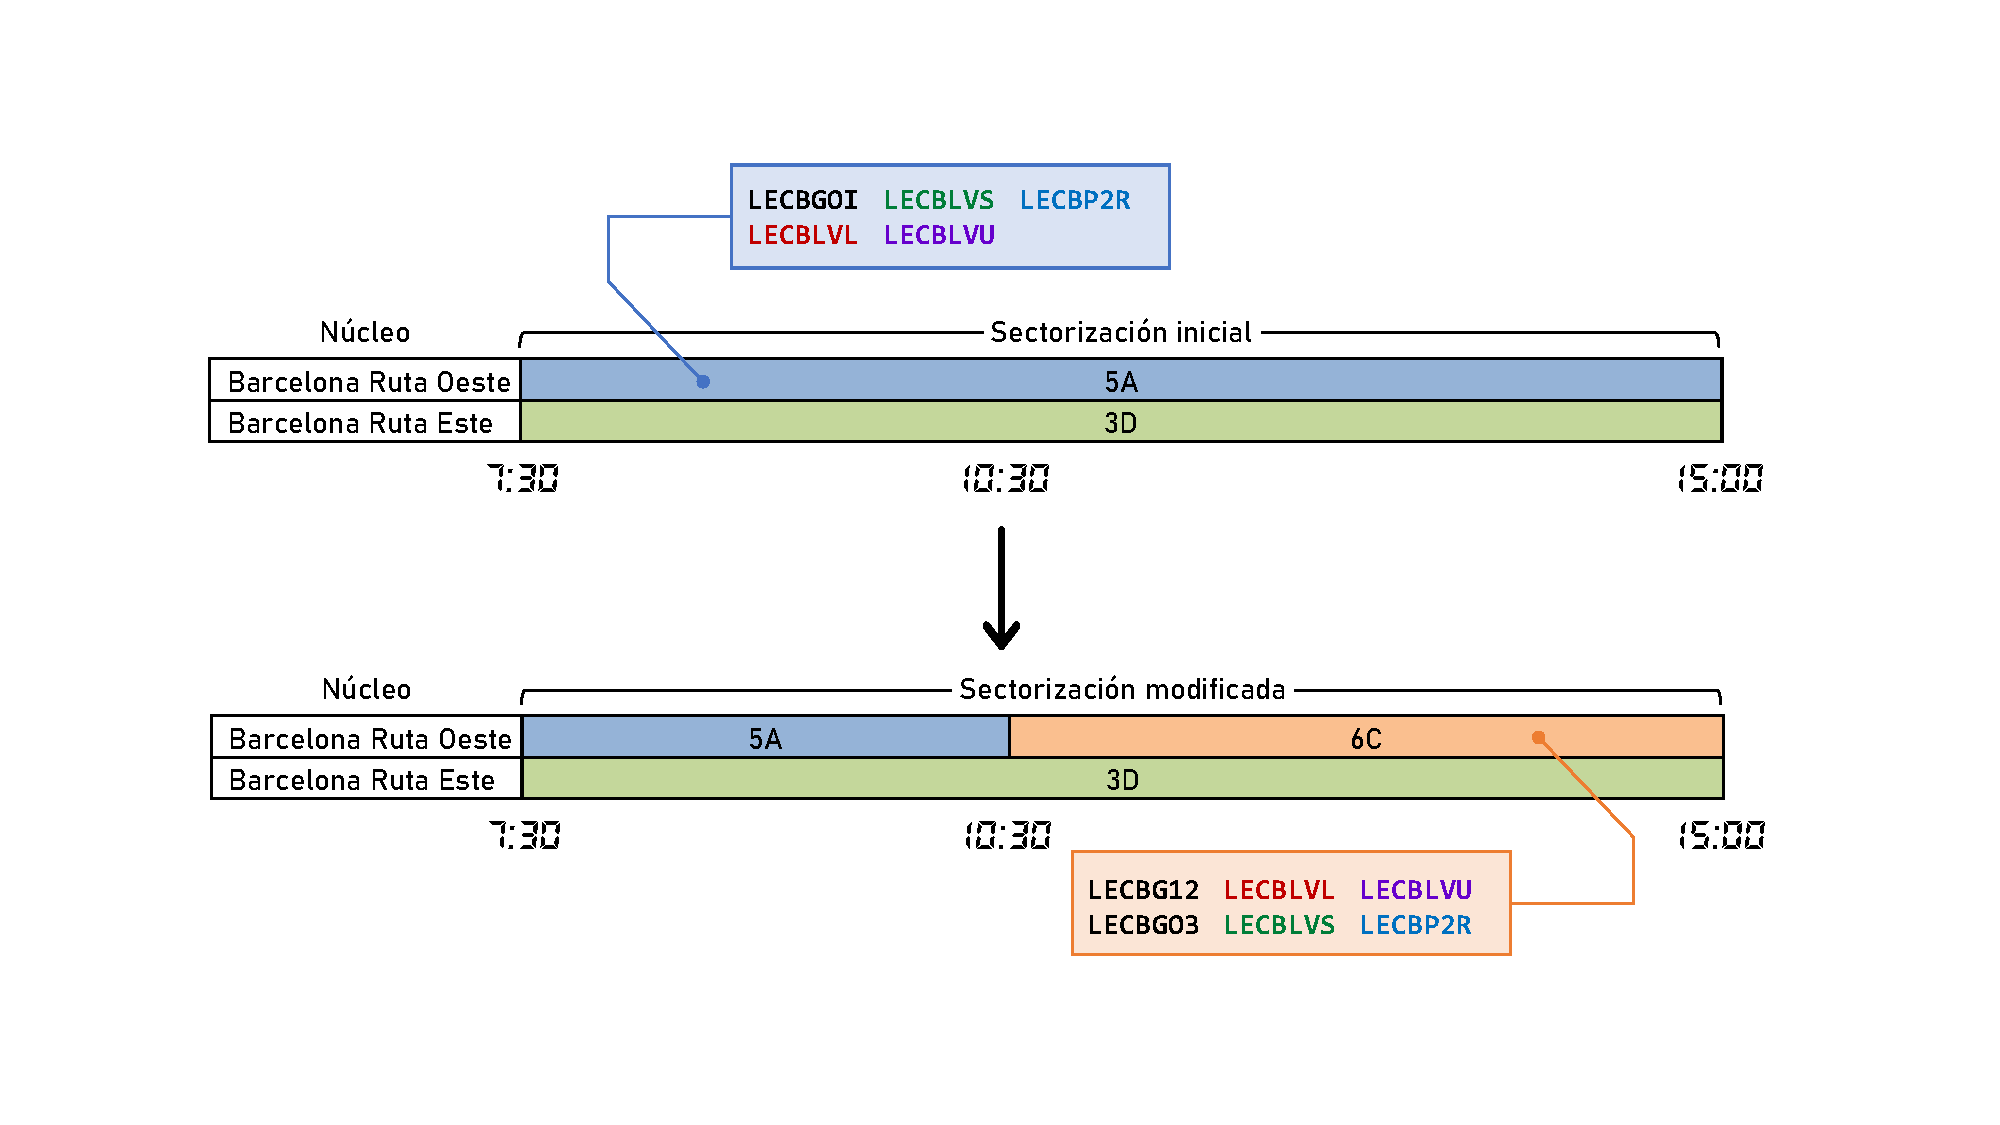
\includegraphics[width=\linewidth]{Ejemplo-cambio-sectorizacion}
	\caption[Ejemplo de cambio de sectorización]{Ejemplo de un posible cambio de sectorización en la Unidad de Control 
	de Barcelona. En color aquellos sectores comunes a ambas sectorizaciones'}
	\label{fig:3:ejemplo-cambio-sectorizacion}
\end{figure}


Identificamos pues, el momento de la incidencia a las 10:30, sin embargo el \textit{momento actual} viene dado a como parte de la entrada. En este caso, han decidido que sea media hora antes de la incidencia, a las 10:00 horas, que equivale al slot número 30:
\[ 
	10 \,h-7 \,h \,30 \,min = 2 \,h \,30 \,min = \left(2 \, \cancel{h} \times \frac{60 \,min}{1 \,\cancel{h}}\right) 
	\,min + 30\,min = 150 
	\,min 
\]

\[
	150 \,\cancel{min} \times \frac{1\,slot}{5\,\cancel{min}} = 30\,slots
\]

Antes de dicha hora, la planificación no debe ser alterada en ningún caso, pues representa el pasado. En la 
\autoref{fig:3:ejemplo-distribucion-inicial} la hemos representado con una línea roja. 

En el resto de la planificación, debemos eliminar todos los sectores que no aparecen. Para ello eliminamos aquellos que no pertenezcan a la intersección entre la nueva sectorización y la antigua (es decir, los que siguen en color negro en la \autoref{fig:3:ejemplo-cambio-sectorizacion}). 
Adicionalmente, para obtener una mejor solución inicial y favorecer así a la búsqueda, en el momento de eliminar un sector de la sectorización inicial, tratamos de sustituirlo por uno de los sectores nuevos que se abren (los de la nueva sectorización, los del cuadro naranja en color negro) \textbf{de forma que sean afines de entre sí}, pues el controlador seguirá pudiendo controlarlo sin problemas de acreditación. %FIXME es esto cierto?

Para hacer más eficiente el recorrido del algoritmo, en lugar de ir slot a slot, podemos agruparlos mientras la sectorización sea la misma. Buscamos un sector afín a cada sector que se cierra y lo sustituimos en todas las apariciones dentro de ese conjunto de slots. Así sucesivamente para cada tramo de slots con la misma sectorización. 
La búsqueda del sector afín es un algoritmo voraz que obtiene el primer sector de entre los que se abren que sea afín al que se cierra, evitando repeticiones.

\begin{algorithm}[H]
%	\SetAlgoLined
	\DontPrintSemicolon
	\KwData{
		
		$Sectorizacion_{inicial} = $ conjunto de sectores de la sectorización inicial para cada slot.
			
		$Sectorizacion_{modificada} = $ conjunto de sectores de la sectorización modificada para cada slot.
	}
	\medskip
	
	\ForEach{conjunto de slots con la misma sectorización}{
		$cerrados \leftarrow { Sectorizacion_{modificada}[slot] \setminus Sectorizacion_{inicial}[slot] }$\;
		$abiertos \leftarrow { Sectorizacion_{inicial}[slot] \setminus Sectorizacion_{modificada}[slot] }$\;
		
		\ForEach{$sector_c \in cerrados$}{
			$afin \leftarrow$ buscarPrimerAfin($Sectorizacion_{modificada}[slot]$)\;
			
			\If{$\nexists{afin}$}{
				$\forall$ aparición de $sector_c$, sustituir por descansos $(111)$\;
			} \Else{
				$\forall$ aparición de $sector_c$, sustituir por $afin$\;
			}
		}
			
	}
	
	\caption{Heurística de inicialización: AFINIDADES}
\end{algorithm}


En nuestro ejemplo, solo tenemos un único sector que se cierra, LECBGOI, que sustituiremos, mediante el algoritmo, por el sector LECBG12, que es el primero afín de entre los nuevos abiertos. Mediante esta heurística, evitaremos tener que añadir plantillas (ver \autoref{apartado:3:paso-2}) de todos los sectores nuevos reutilizando los controladores ya existentes.

\subsubsection{Paso 2: Introducir plantillas de los nuevos sectores} \label{apartado:3:paso-2}

Partimos de la lista de sectores nuevos que se abren y que no han sido ya empleados en el paso anterior como sustituto de alguno de los que se cierran. Lo que haremos será añadir a la planificación una plantilla $3\times1$ como la de la 
\autoref{fig:3:plantilla-3x1} donde alternamos trabajo y descanso a tamaños iguales: el doble de trabajo (uno en cada puesto) por cada uno de descanso. Las plantillas pueden emplearse con cualquier escala de tiempo, manteniendo las proporciones, por ejemplo 2 horas de trabajo y una de descanso.
Para este proyecto se ha utilizado un tamaño de 6 slots de descanso (12 de trabajo) debido a que los resultados eran mejores empleando esta proporción en proyectos previos a la presente tesis, por lo que se ha mantenido dicha proporción.

\begin{figure}
	\centering
	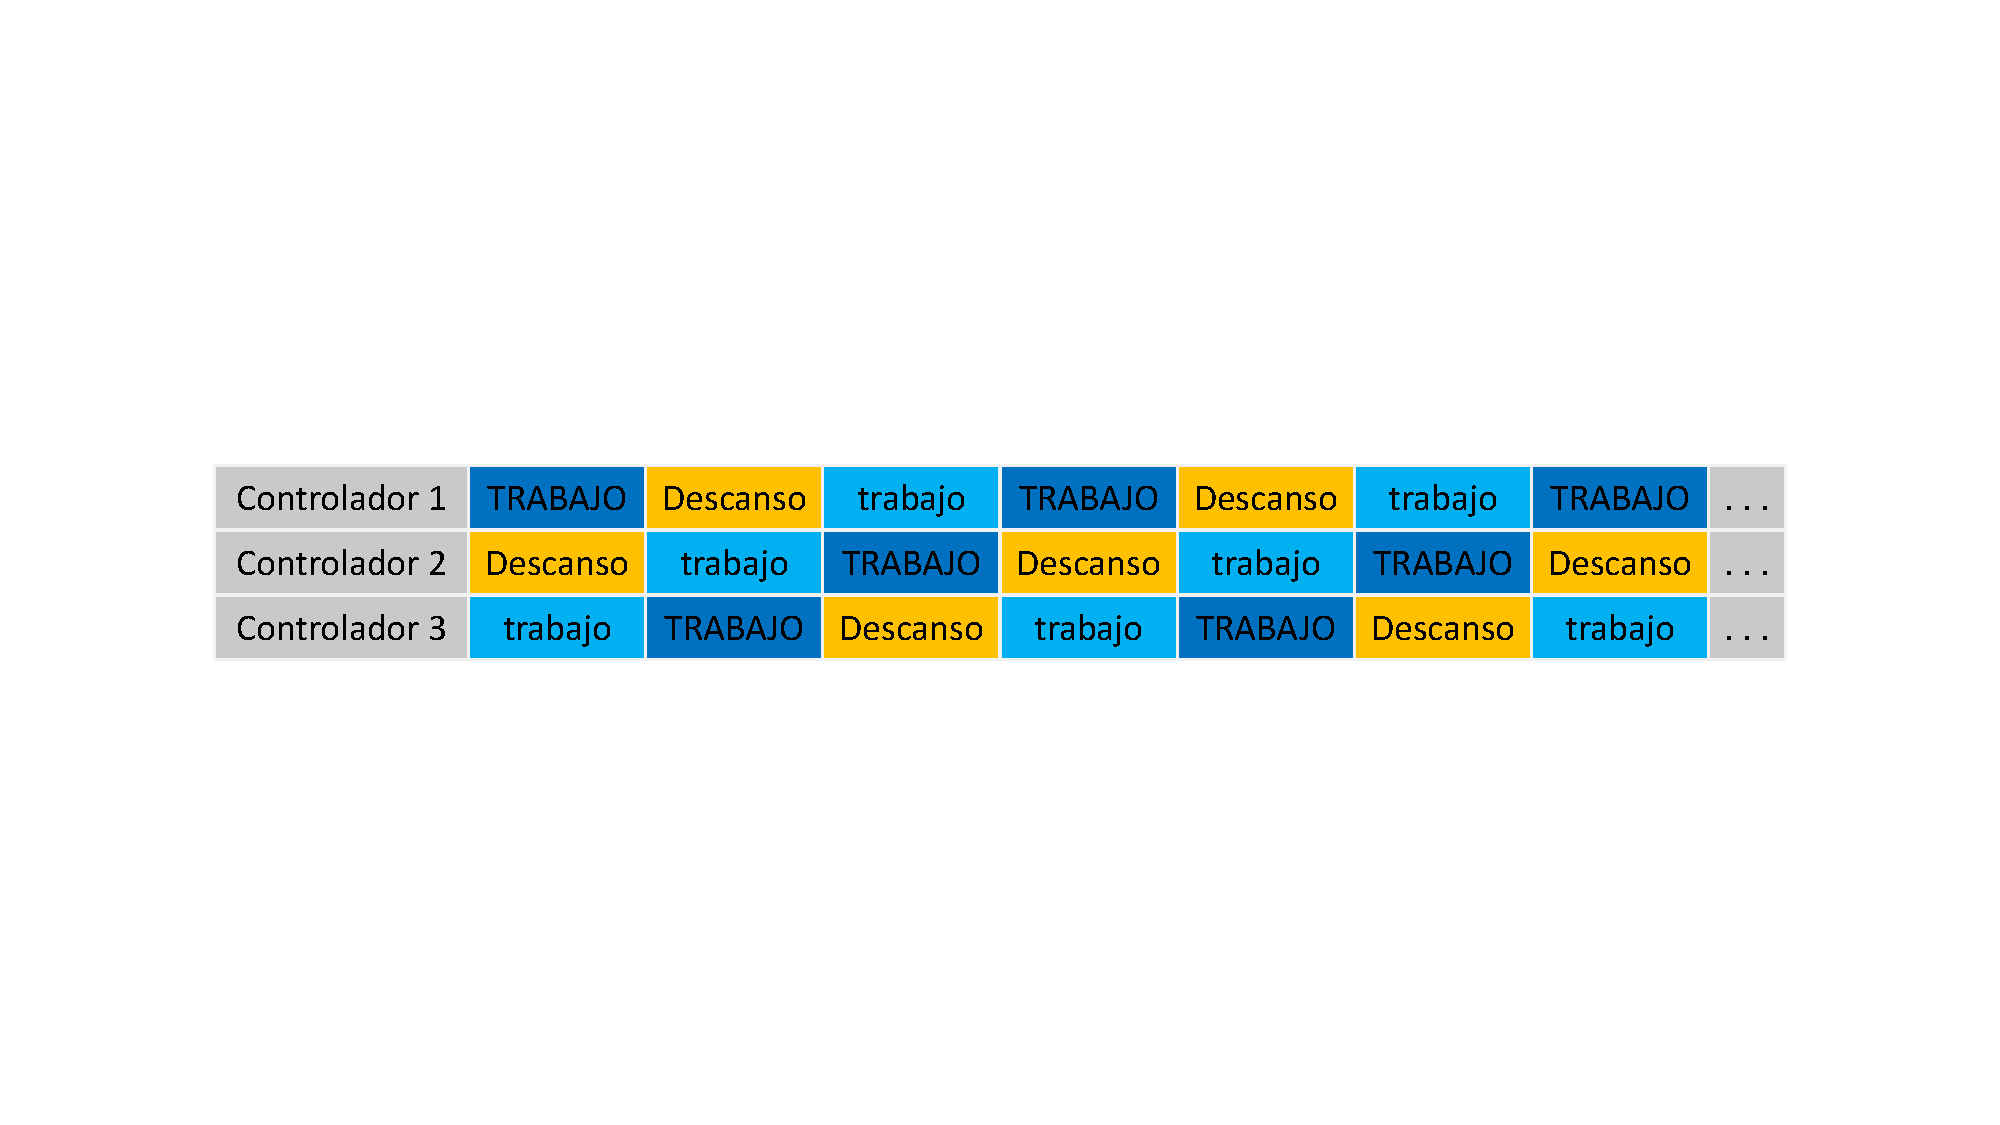
\includegraphics[width=0.9\linewidth]{capitulos/Capitulo3-Metodologia-propuesta/recursos/Plantilla-3x1}
	\caption[Aspecto de una plantilla 3x1]{Aspecto de una plantilla 3x1. Las letras mayúsculas representan trabajo en 
	puesto ejecutivo y las minúsculas en planificador.}
	\label{fig:3:plantilla-3x1}
\end{figure}

De esta forma, obtendremos una planificación en la que se han tenido en cuenta las contingencias relativas a los cambios de sectorización. Si la instancia concreta del problema incluye únicamente esta incidencia, la planificación de la \autoref{fig:3:ejemplo-distribucion-pasos-1-y-2} sería una \textit{solución inicial} preparada para emplear como entrada a la \fasedos{}.

\begin{figure} 
	\centering
	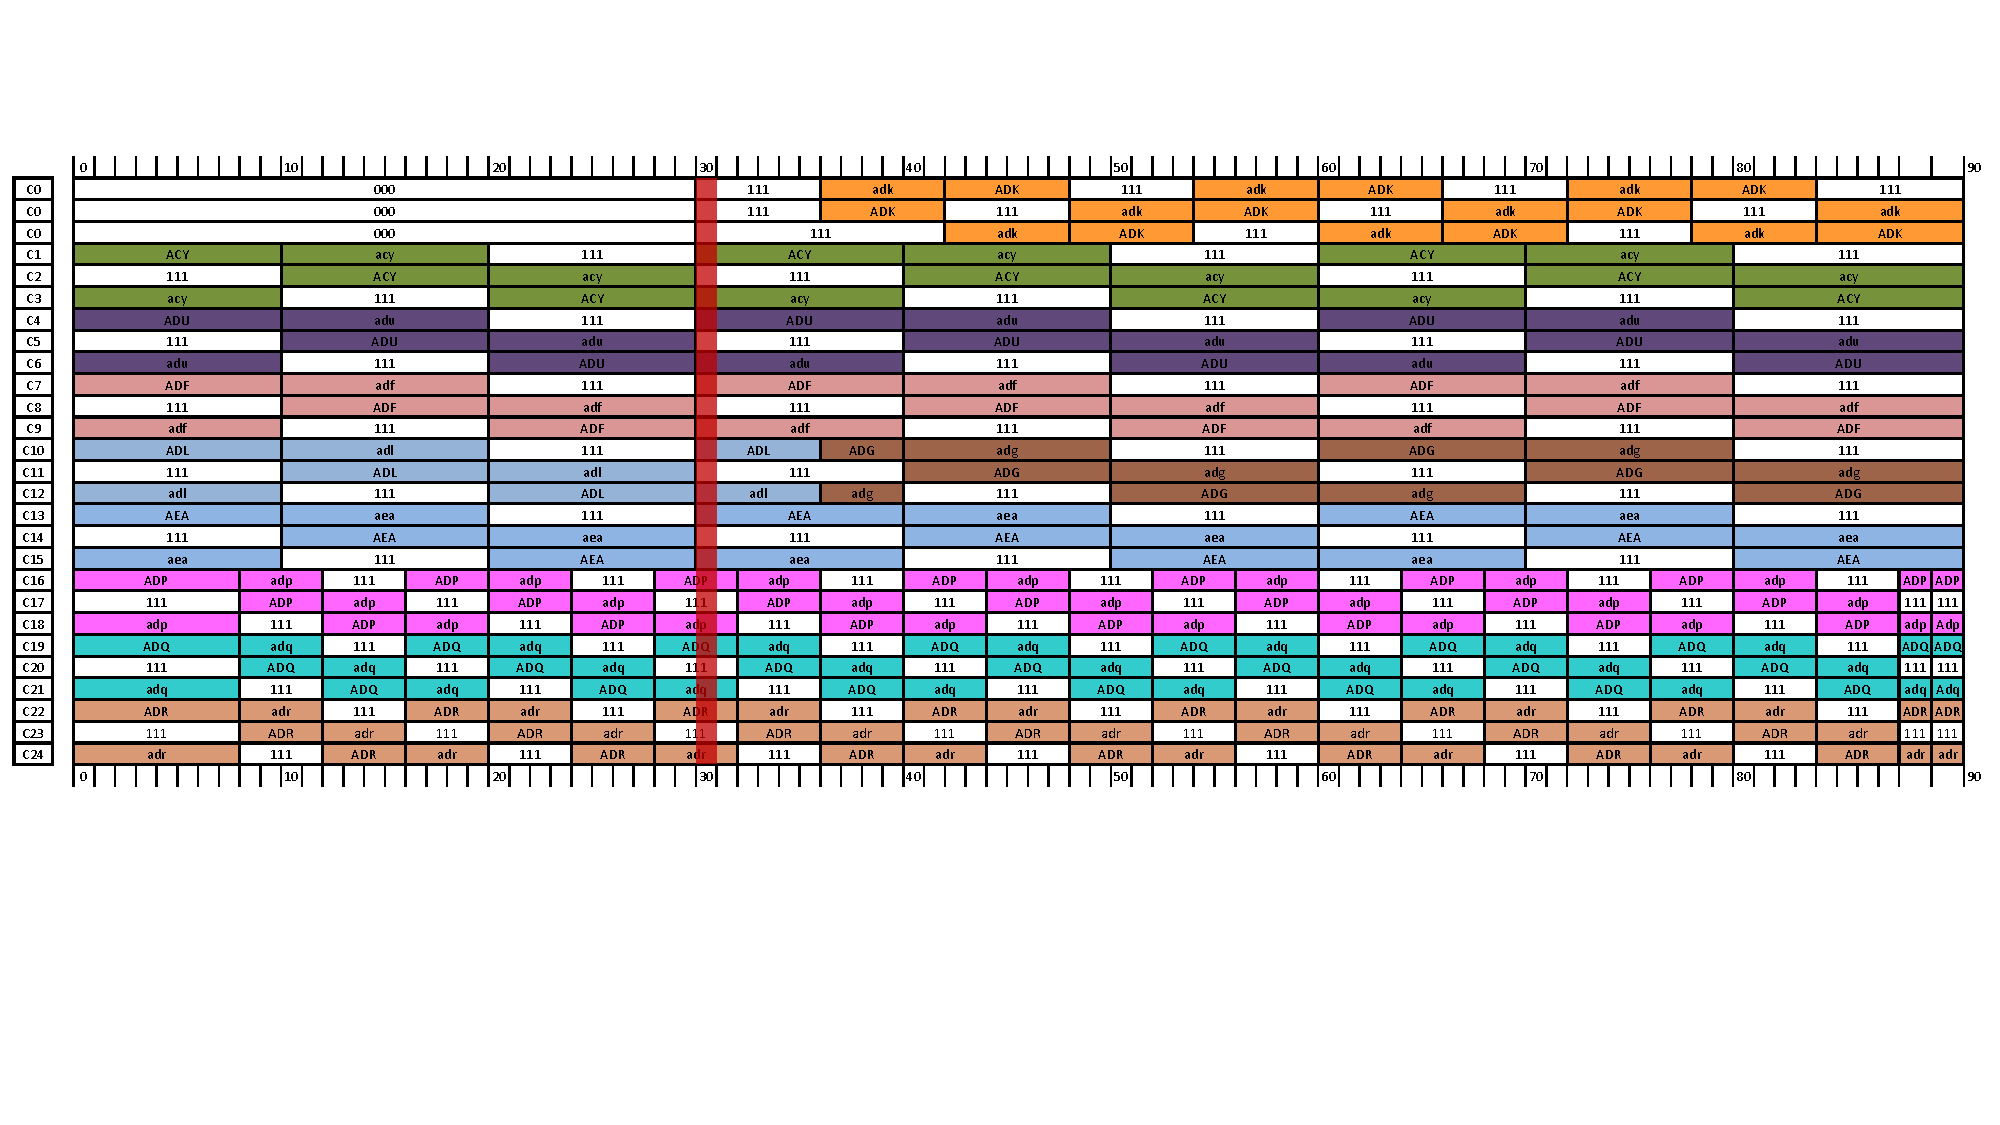
\includegraphics[width=\linewidth]{Ejemplo-distribucion-pasos-1-y-2}
	\caption[Planificación tras los pasos 1 y 2 de la Fase 1]{Planificación tras los pasos 1 y 2 de la \faseuno{} siguiendo el ejemplo de la \autoref{fig:3:ejemplo-distribucion-inicial}. Los controladores con identificador C0 son imaginarios, es decir no existen pero son necesarios en la inicialización y deberán ser eliminador en la \fasedos{}} 
	\label{fig:3:ejemplo-distribucion-pasos-1-y-2}
\end{figure}

\subsubsection{Paso 3 y 4: Dar de baja/alta a los controladores}
Estos pasos son ejecutados únicamente en caso de que haya una incidencia relacionada con el personal. Podría suceder que tras ponerse de baja repentinamente, otro controlador cubra ese puesto a lo largo de la jornada, por lo que tendremos que hacer dos modificaciones a la planificación:

El controlador que se da de baja dejará de trabajar ese día, sin embargo no podemos eliminarlo de la planificación puesto que en momentos previos al \textit{momento actual} si ha trabajado, y hemos de contabilizarlo como carga de trabajo. Emplearemos el carácter especial ``000'' para indicar que se trata de un slot en el que el controlador no está trabajando pero tampoco descansado, al que se deberá tratar de forma especial durante la ejecución de la \fasedos{}, pues no se podrá mover a otro controlador ni se le podrá asignar nuevo trabajo. Si ningún trabajador se reincorpora a su puesto de trabajo, emplearemos un controlador imaginario al que se le asignará toda la carga de trabajo que tenía en controlador de baja a partir del momento de la incidencia. La \autoref{fig:3:ejemplo-distribucion-pasos-3-y-4} muestra un ejemplo donde el controlador 23 se ha puesto de baja a las 9:30 (slot 30) y no hay reincorporación (en caso de haberla el controlador $C_0$ tendría su identificador correspondiente). Nótese que se emplean los caracteres de fuera de turno (``000'') en todos los slots a partir de la incidencia en el caso del controlador de baja mientras que para el controlador imaginario (o el reincorporado según se aplique) sucede lo contrario: todos los slots previos a la incidencia tienen el mencionado carácter. 
% Se tratan de slots inalterables en todos los casos, pero a la hora de contabilizarse el trabajo (ver Fitness) %TODO referencia no se han de computar como tiempo de descanso

\begin{figure}
	\centering
	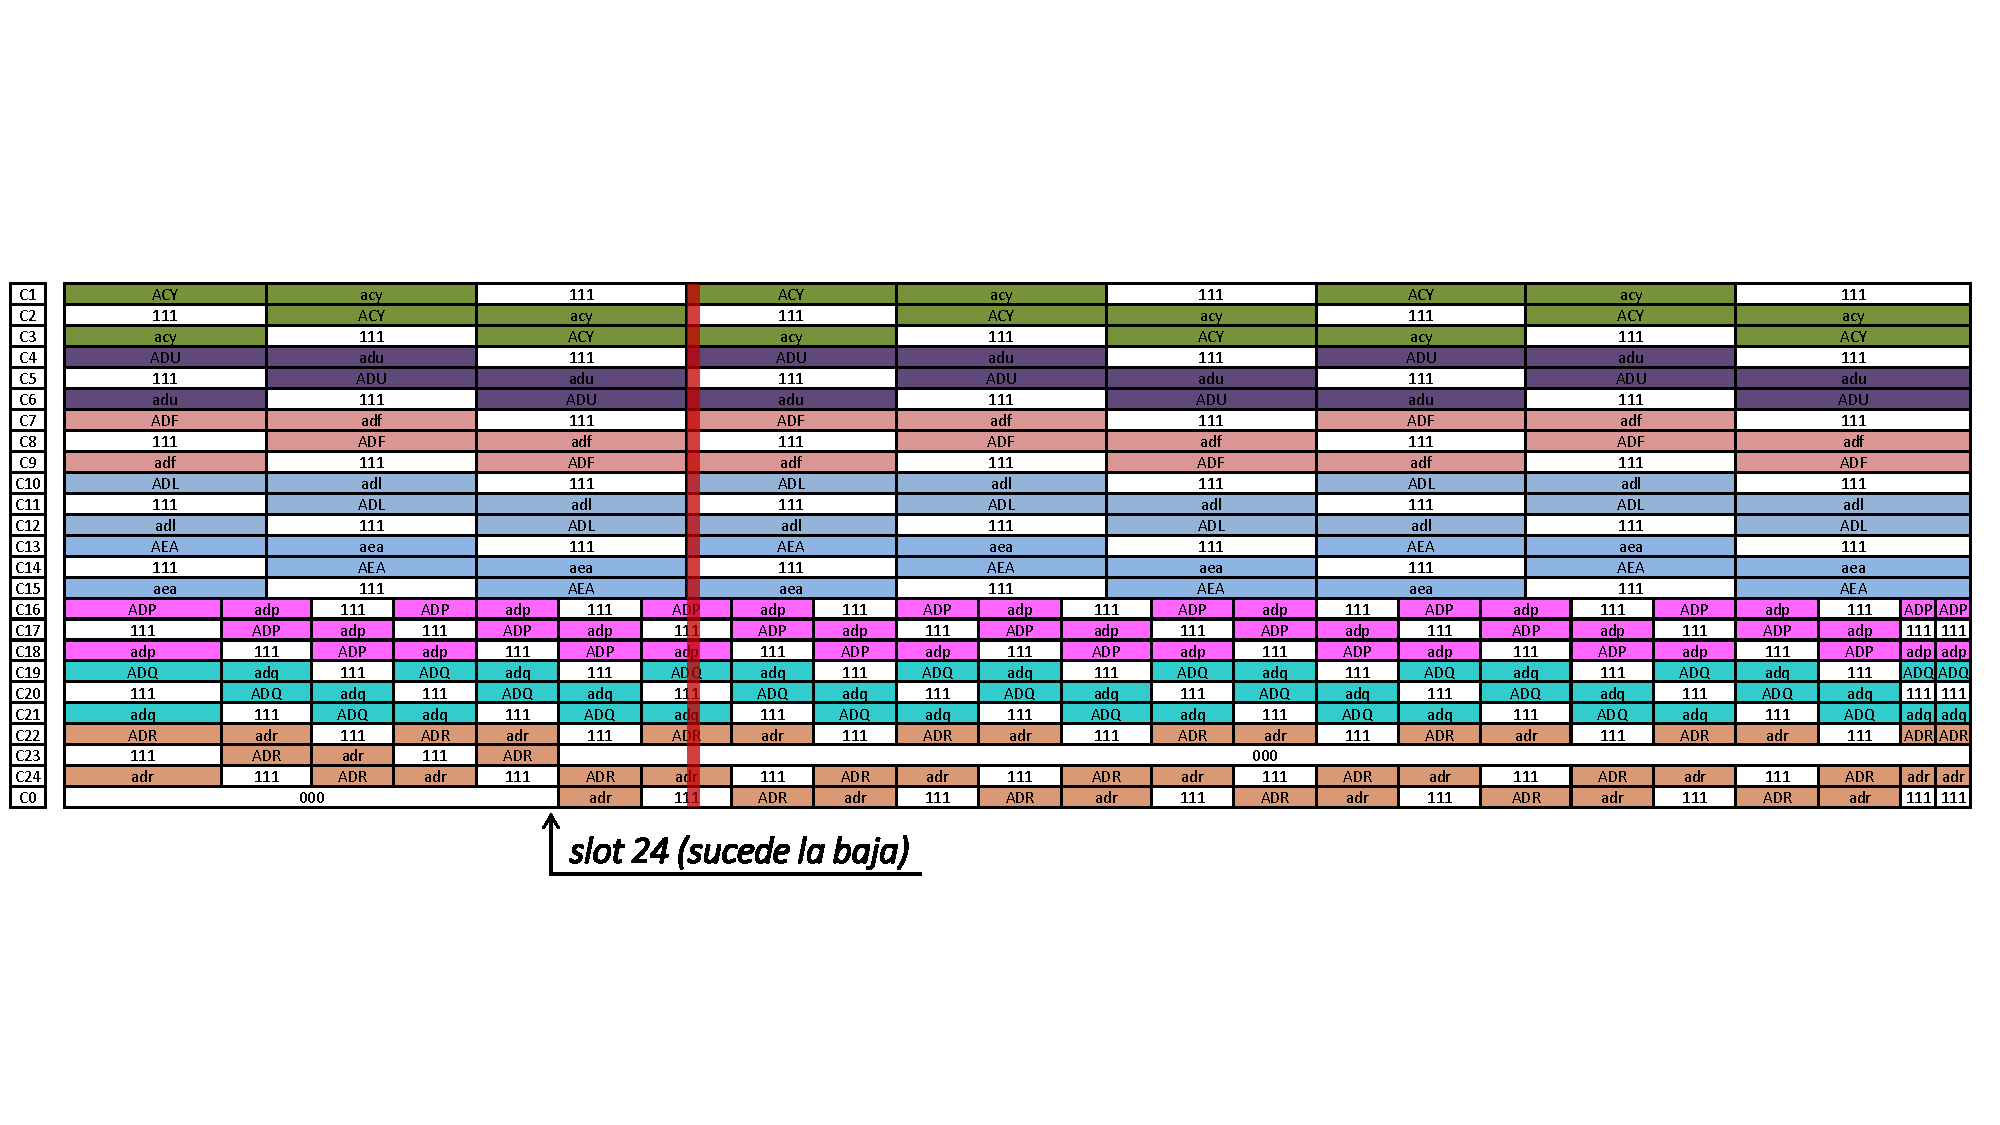
\includegraphics[width=\linewidth]{Ejemplo-distribucion-pasos-3-y-4}
	\caption[Ejemplo de planificación tras los pasos 3 y 4 de la \faseuno{}]{Ejemplo de planificación tras los pasos 3 y 4 de la \faseuno{}. En este caso no ha habido reincorporaciones}
	\label{fig:3:ejemplo-distribucion-pasos-3-y-4}
\end{figure}

